\documentclass[11pt]{article}
\usepackage[utf8]{inputenc}
\usepackage[T1]{fontenc}
\usepackage{amsmath,amssymb}
\usepackage{graphicx}
\usepackage{xcolor}
\usepackage{booktabs}
\usepackage[margin=2.1cm]{geometry}
\usepackage{array}
\usepackage{fancyhdr}

\definecolor{azul}{RGB}{0,70,140}

\newcommand{\seccion}[1]{%
  \vspace{4pt}\noindent{\color{azul}\large\bfseries #1}\par\vspace{2pt}\hrule\vspace{6pt}}

\pagestyle{fancy}\fancyhf{}
\rhead{\small Modelado y Simulación}
\lhead{\small Resolución de examen — Parte 2}
\cfoot{\thepage}

\setlength{\parindent}{0pt}
\setlength{\parskip}{4pt}

\begin{document}

\begin{center}
  {\color{azul}\LARGE\bfseries Resolución completa del examen (Parte 2)}\\[2pt]
  {\large Sistemas dinámicos — Docente: Omar Cáceres}\\[2pt]
  \rule{\textwidth}{0.8pt}
\end{center}

%==================================================================
\seccion{Ejercicio 1 — Modelo logístico (saturación de un servidor)}

\[
\dot{x}=r\,x\!\left(1-\frac{x}{k}\right),\qquad
k=20000\ \text{rps},\quad r=0.15\ \text{min}^{-1},\quad x_0=1500\ \text{rps}.
\]

\textbf{Puntos de equilibrio.} $\dot x=0\Rightarrow r\,x\!\left(1-\dfrac{x}{k}\right)=0$:
\[
\boxed{x_1^{*}=0}\qquad\text{y}\qquad \boxed{x_2^{*}=k=20000}.
\]
\textbf{Estabilidad} (signo de $f'(x)$ con $f(x)=rx-\dfrac{r}{k}x^2$, $f'(x)=r-\dfrac{2r}{k}x$):
\[
f'(0)=r=0.15>0\ \Rightarrow\ x=0\ \text{INESTABLE};\qquad
f'(k)=r-2r=-r<0\ \Rightarrow\ x=k\ \text{ESTABLE}.
\]

\textbf{a) Solución analítica} (variables separables):
\[
\frac{dx}{x\left(1-\frac{x}{k}\right)}=r\,dt.
\]
Fracciones simples: $\dfrac{1}{x\left(1-\frac{x}{k}\right)}=\dfrac{1}{x}+\dfrac{1}{k-x}$. Integrando:
\[
\int\!\left(\frac{1}{x}+\frac{1}{k-x}\right)dx=\int r\,dt
\ \Rightarrow\ \ln|x|-\ln|k-x|=rt+C
\ \Rightarrow\ \ln\!\frac{x}{k-x}=rt+C.
\]
Despejando ($e^{C}$ constante) e invirtiendo:
\[
\frac{k-x}{x}=e^{-C}e^{-rt}\ \Rightarrow\ \frac{k}{x}-1=e^{-C}e^{-rt}
\ \Rightarrow\ \boxed{\,x(t)=\frac{k}{1+A\,e^{-rt}}\,},\quad
\boxed{A=\frac{k-x_0}{x_0}}.
\]
Con los datos: $A=\dfrac{20000-1500}{1500}=\dfrac{18500}{1500}=\dfrac{37}{3}\approx 12.33$.

\textbf{Comprobación de la condición inicial:} $x(0)=\dfrac{k}{1+A}=\dfrac{20000}{1+37/3}=\dfrac{20000}{40/3}=1500=x_0.\ \checkmark$

\textbf{b) Tiempo de saturación.} El servidor ``satura'' en el punto de inflexión de la curva
logística, donde la tasa de crecimiento es máxima: $x=\dfrac{k}{2}$. Imponiendo $x(t_s)=\dfrac{k}{2}$:
\[
\frac{k}{1+A e^{-rt_s}}=\frac{k}{2}\ \Rightarrow\ 1+Ae^{-rt_s}=2\ \Rightarrow\ Ae^{-rt_s}=1
\ \Rightarrow\ e^{rt_s}=A.
\]
\[
\Rightarrow\ \boxed{\,t_s=\frac{1}{r}\ln A=\frac{1}{r}\ln\!\left(\frac{k-x_0}{x_0}\right)}.
\]
Cálculo numérico:
\[
t_s=\frac{1}{0.15}\,\ln\!\left(\frac{18500}{1500}\right)=6.6\overline{6}\cdot\ln(12.33)
=6.6\overline{6}\cdot 2.512=\boxed{16.75\ \text{min}}.
\]

\begin{figure}[htbp]\centering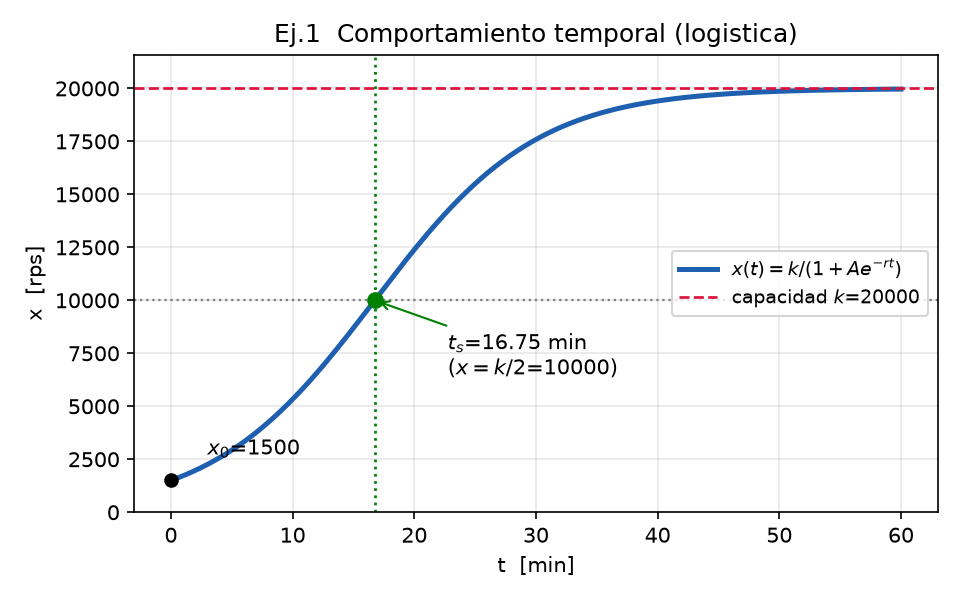
\includegraphics[width=0.74\textwidth]{ej1_temporal.png}\end{figure}

\textbf{Diagrama de fase (1D) y de bifurcación.} En la línea de fase, $\dot x>0$ para $0<x<k$
(crece hacia $k$) y $\dot x<0$ para $x>k$: confirma $x=k$ estable y $x=0$ inestable.
Tomando $r$ como parámetro de control se obtiene una \textbf{bifurcación transcrítica} en $r=0$:
las ramas $x^{*}=0$ y $x^{*}=k$ \emph{intercambian su estabilidad} al cambiar el signo de $r$.

\begin{figure}[htbp]\centering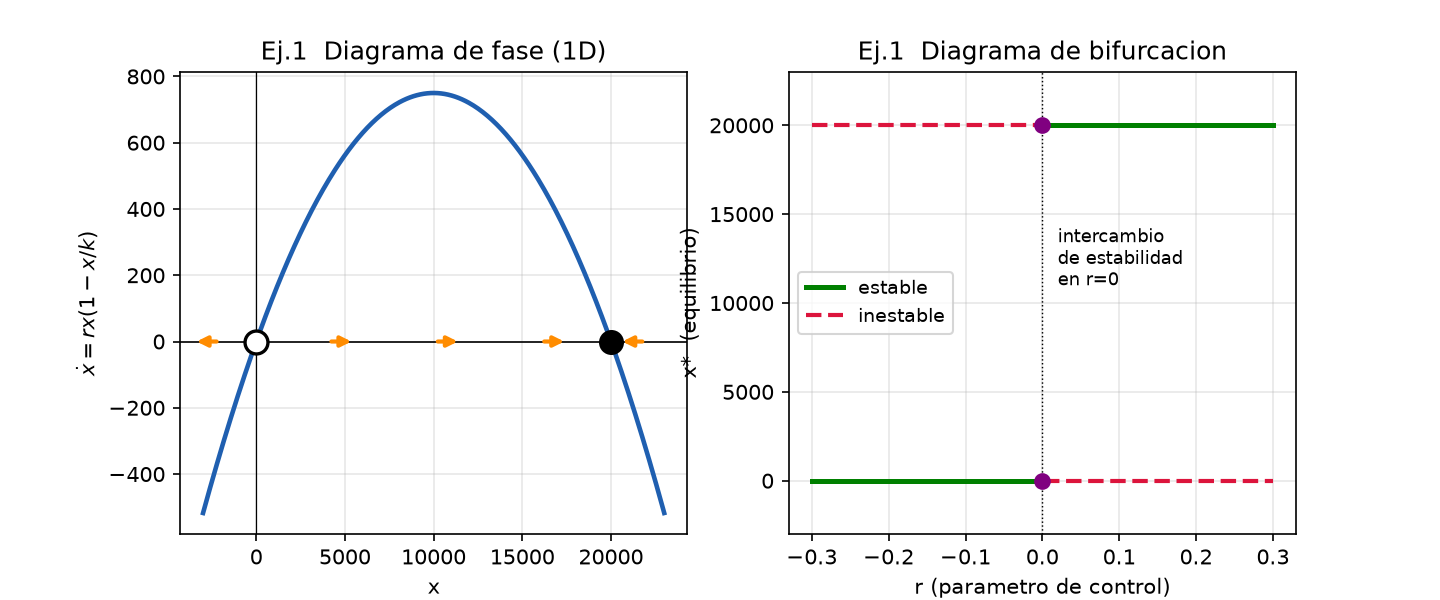
\includegraphics[width=0.98\textwidth]{ej1_fase_bif.png}\end{figure}

\newpage
%==================================================================
\seccion{Ejercicio 2 — Sistema lineal $\dot x=x+2y,\ \dot y=4x+3y$}

\[
\dot{\vec x}=A\vec x,\qquad A=\begin{pmatrix}1 & 2\\ 4 & 3\end{pmatrix}.
\]

\textbf{c) Autovalores.} $\det(A-\lambda I)=0$:
\[
\det\!\begin{pmatrix}1-\lambda & 2\\ 4 & 3-\lambda\end{pmatrix}
=(1-\lambda)(3-\lambda)-8=\lambda^2-4\lambda-5=0.
\]
\[
\lambda=\frac{4\pm\sqrt{16+20}}{2}=\frac{4\pm6}{2}
\ \Rightarrow\ \boxed{\lambda_1=5,\quad \lambda_2=-1}.
\]
Reales de signo opuesto $\Rightarrow$ el origen es un \textbf{PUNTO SILLA}.

\textbf{Autovectores.}
\[
\lambda_1=5:\ (A-5I)\vec v=\begin{pmatrix}-4 & 2\\ 4 & -2\end{pmatrix}\vec v=0
\Rightarrow -4v_1+2v_2=0\Rightarrow v_2=2v_1\Rightarrow \boxed{\vec v_1=(1,2)}\ (\text{inestable}).
\]
\[
\lambda_2=-1:\ (A+I)\vec v=\begin{pmatrix}2 & 2\\ 4 & 4\end{pmatrix}\vec v=0
\Rightarrow v_2=-v_1\Rightarrow \boxed{\vec v_2=(1,-1)}\ (\text{estable}).
\]

\textbf{Solución general.}
\[
\vec x(t)=c_1e^{5t}\begin{pmatrix}1\\2\end{pmatrix}+c_2e^{-t}\begin{pmatrix}1\\-1\end{pmatrix}
\ \Rightarrow\
\boxed{x(t)=c_1e^{5t}+c_2e^{-t}},\quad \boxed{y(t)=2c_1e^{5t}-c_2e^{-t}}.
\]

\textbf{d) Nulclinas.}
\[
\dot x=0:\ x+2y=0\Rightarrow \boxed{y=-\tfrac{x}{2}}\quad(\text{campo vertical}),
\]
\[
\dot y=0:\ 4x+3y=0\Rightarrow \boxed{y=-\tfrac{4x}{3}}\quad(\text{campo horizontal}).
\]

\begin{figure}[htbp]\centering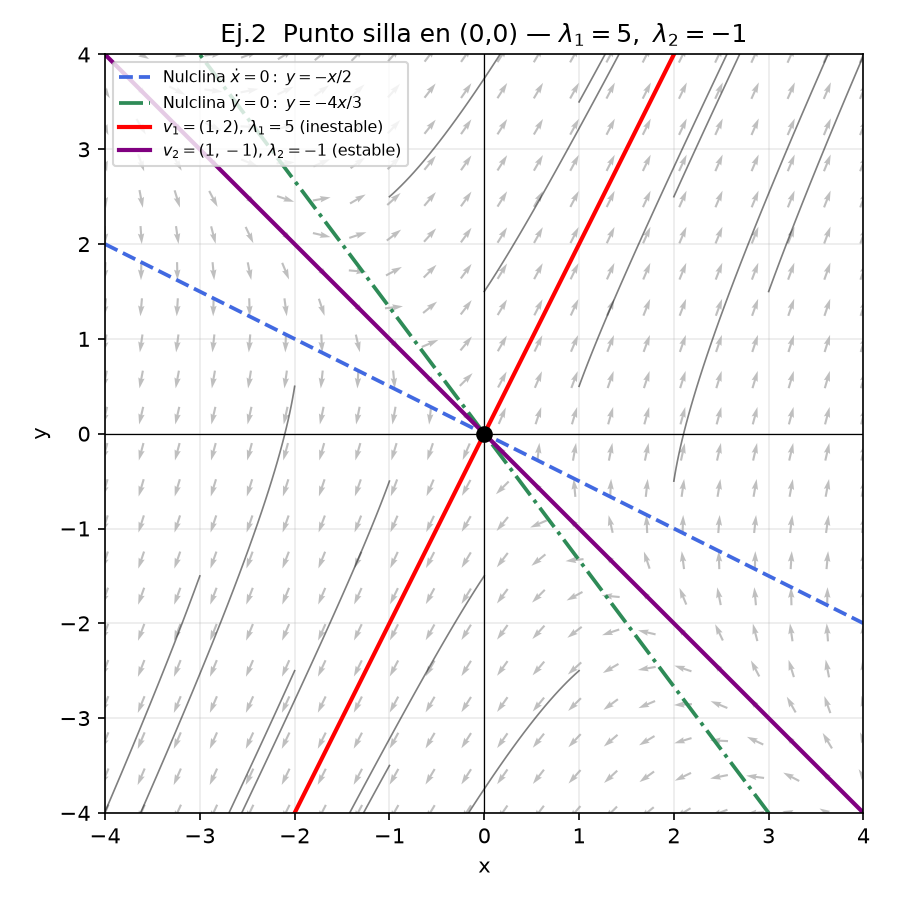
\includegraphics[width=0.60\textwidth]{ej2_silla.png}\end{figure}

\newpage
%==================================================================
\seccion{Ejercicio 3 — No lineal $\dot x=y,\ \dot y=x^2+y^2-1$}

\textbf{a) ¿Es conservativo?} Un sistema $\dot{\vec x}=\vec F$ es conservativo (preserva áreas en
el espacio de fases) si y solo si su \textbf{divergencia es nula}:
\[
\nabla\!\cdot\vec F=\frac{\partial \dot x}{\partial x}+\frac{\partial \dot y}{\partial y}
=\frac{\partial (y)}{\partial x}+\frac{\partial (x^2+y^2-1)}{\partial y}
=0+2y=2y.
\]
\[
\boxed{\nabla\!\cdot\vec F=2y\neq 0\ \Rightarrow\ \textbf{NO es conservativo}.}
\]
(Equivalente: un sistema mecánico conservativo tiene la forma $\dot x=y,\ \dot y=f(x)$ con energía
$E=\tfrac12 y^2-\!\int\! f\,dx$; aquí $\dot y=x^2+y^2-1$ \emph{depende de} $y$, así que no admite esa energía.)
El sistema contrae áreas donde $y<0$ y las expande donde $y>0$.

\textbf{b) Diagrama de fase.} \emph{Equilibrios:} $\dot x=0\Rightarrow y=0$; con $y=0$,
$\dot y=x^2-1=0\Rightarrow x=\pm1$:
\[
\boxed{P_1=(1,0)}\qquad\text{y}\qquad\boxed{P_2=(-1,0)}.
\]
\emph{Jacobiano:}
\[
J(x,y)=\begin{pmatrix} 0 & 1\\ 2x & 2y\end{pmatrix}.
\]
\[
J(1,0)=\begin{pmatrix}0&1\\2&0\end{pmatrix}:\ \operatorname{tr}=0,\ \det=-2
\Rightarrow \lambda=\pm\sqrt2\ \Rightarrow\ \boxed{P_1\ \text{SILLA}}.
\]
\[
J(-1,0)=\begin{pmatrix}0&1\\-2&0\end{pmatrix}:\ \operatorname{tr}=0,\ \det=2
\Rightarrow \lambda=\pm\sqrt2\,i\ \Rightarrow\ \boxed{P_2\ \text{CENTRO}}.
\]
\emph{Observación} (justifica las órbitas cerradas): el sistema es \textbf{reversible} ante
$(y,t)\to(-y,-t)$ y $P_2$ está sobre el eje de simetría $\Rightarrow$ $(-1,0)$ es un centro genuino:
las trayectorias a su alrededor son curvas cerradas. La órbita que pasa por la silla $(1,0)$ es la
\emph{separatriz} (lazo homoclínico) que encierra a esas órbitas.

\begin{figure}[htbp]\centering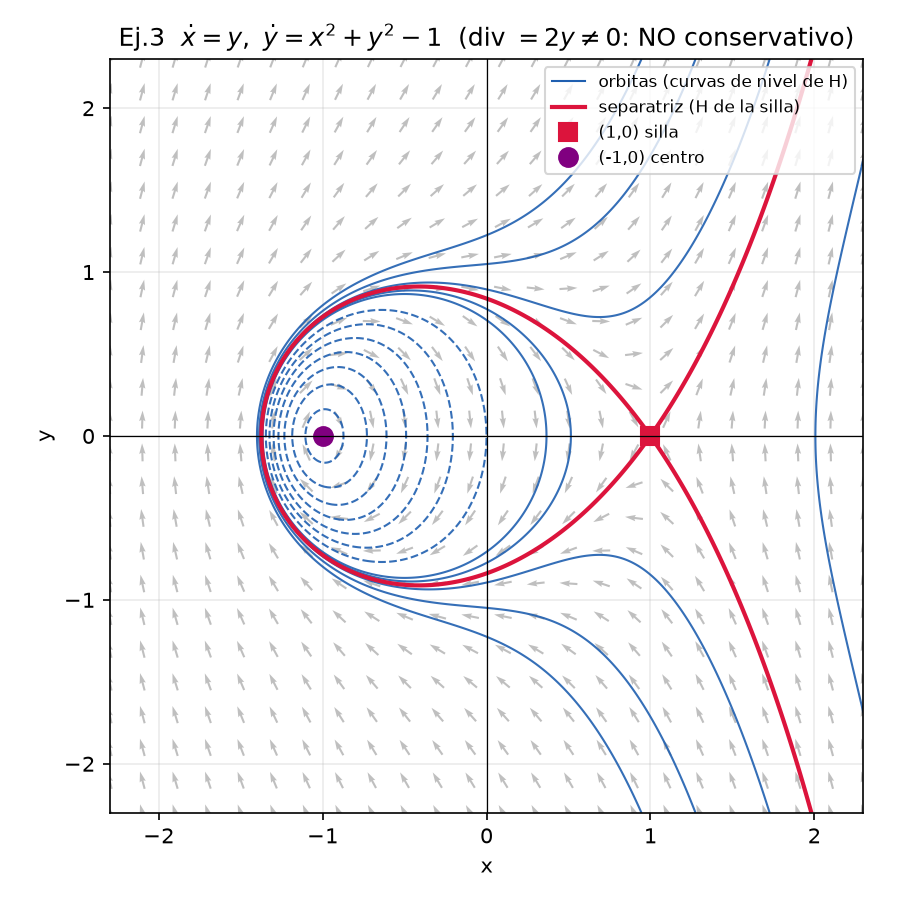
\includegraphics[width=0.62\textwidth]{ej3_noconserv.png}\end{figure}

\newpage
%==================================================================
\seccion{Ejercicio 4 — Competencia Lotka–Volterra}

\[
\begin{cases}\dot x=x(2-x-y)\\[2pt]\dot y=y(3-2x-y)\end{cases}
\qquad x=\text{conejos},\ \ y=\text{ovejas}\ (x,y\ge0).
\]

\textbf{a) Puntos críticos.} Anulando ambas ecuaciones se obtienen cuatro equilibrios:
\[
\boxed{(0,0)},\quad \boxed{(2,0)},\quad \boxed{(0,3)},\quad
\boxed{(1,1)}\ \big(\text{de } 2-x-y=0\ \text{y}\ 3-2x-y=0\big).
\]

\emph{Jacobiano} (con $\dot x=2x-x^2-xy,\ \dot y=3y-2xy-y^2$):
\[
J(x,y)=\begin{pmatrix} 2-2x-y & -x\\ -2y & 3-2x-2y\end{pmatrix}.
\]

\textbf{Clasificación de cada punto:}
\[
J(0,0)=\begin{pmatrix}2&0\\0&3\end{pmatrix}\Rightarrow \lambda=2,3>0
\ \Rightarrow\ \boxed{(0,0)\ \text{NODO INESTABLE (fuente)}};\quad \vec v=(1,0),(0,1).
\]
\[
J(2,0)=\begin{pmatrix}-2&-2\\0&-1\end{pmatrix}\Rightarrow \lambda=-2,-1<0
\ \Rightarrow\ \boxed{(2,0)\ \text{NODO ESTABLE}};\quad \vec v=(1,0),(2,-1).
\]
\[
J(0,3)=\begin{pmatrix}-1&0\\-6&-3\end{pmatrix}\Rightarrow \lambda=-1,-3<0
\ \Rightarrow\ \boxed{(0,3)\ \text{NODO ESTABLE}};\quad \vec v=(1,-3),(0,1).
\]
Para el punto de coexistencia:
\[
J(1,1)=\begin{pmatrix}-1&-1\\-2&-1\end{pmatrix}:\ \operatorname{tr}=-2,\ \det=1-2=-1<0
\ \Rightarrow\ \boxed{(1,1)\ \text{PUNTO SILLA}}.
\]
\[
\lambda=\frac{-2\pm\sqrt{4-4(-1)}}{2}=-1\pm\sqrt2
\ \Rightarrow\ \lambda_1=-1+\sqrt2\approx0.41>0,\quad \lambda_2=-1-\sqrt2\approx-2.41<0.
\]
Autovectores en $(1,1)$: $\ \lambda_1\!:\ \vec v_1=(1,-\sqrt2)$ (inestable);\quad
$\lambda_2\!:\ \vec v_2=(1,\sqrt2)$ (estable).

\textbf{b) Retrato de fase y regiones.} La \textbf{variedad estable} de la silla $(1,1)$ (dirección
$\vec v_2=(1,\sqrt2)$) es la \textbf{separatriz} que divide el primer cuadrante en dos cuencas de atracción.
Como el punto de coexistencia es inestable (silla), \textbf{no hay coexistencia}: una especie excluye a la
otra (\emph{principio de exclusión competitiva}).
\begin{itemize}
  \item Por \textbf{debajo/derecha} de la separatriz: las trayectorias van a $(2,0)$ $\Rightarrow$
        \textbf{prevalecen los conejos} (las ovejas se extinguen).
  \item Por \textbf{encima/izquierda} de la separatriz: las trayectorias van a $(0,3)$ $\Rightarrow$
        \textbf{prevalecen las ovejas} (los conejos se extinguen).
\end{itemize}

\begin{figure}[htbp]\centering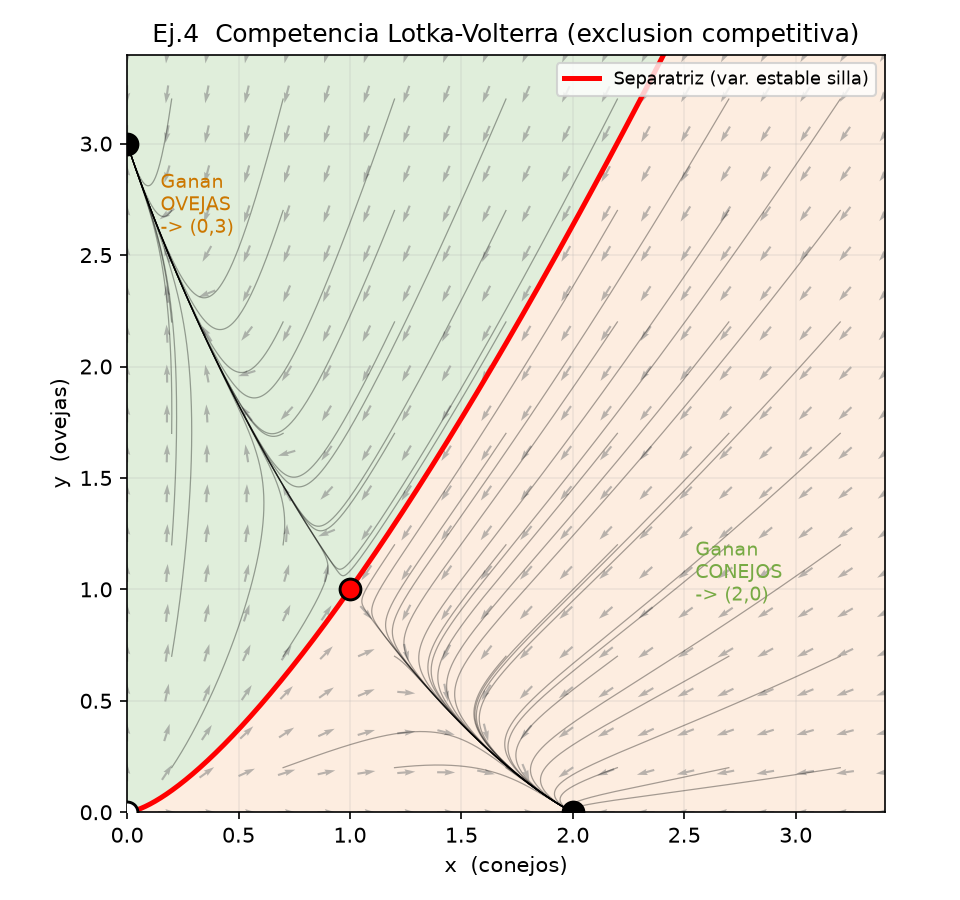
\includegraphics[width=0.66\textwidth]{ej4_lotka.png}\end{figure}

\newpage
%==================================================================
\seccion{Ejercicio 5 — Lyapunov y coordenadas polares}

\[
\begin{cases}\dot x=-y-x(x^2+y^2)\\[2pt]\dot y=\ \ x-y(x^2+y^2)\end{cases}
\qquad\text{único equilibrio: } (0,0).
\]

\textbf{a) Función de Lyapunov} $V(x,y)=\tfrac12 x^2+\tfrac12 y^2$ (definida positiva, $V(0,0)=0$).
Derivada a lo largo de las trayectorias:
\[
\dot V=\frac{\partial V}{\partial x}\dot x+\frac{\partial V}{\partial y}\dot y=x\dot x+y\dot y.
\]
\[
x\dot x=x\big[-y-x(x^2+y^2)\big]=-xy-x^2(x^2+y^2),
\]
\[
y\dot y=y\big[\,x-y(x^2+y^2)\big]=\ \ xy-y^2(x^2+y^2).
\]
Sumando (los términos $\pm xy$ se cancelan):
\[
\dot V=-(x^2+y^2)(x^2+y^2)=\boxed{-(x^2+y^2)^2\le 0},
\]
y $\dot V=0$ solo en el origen. Como $V$ es definida positiva y $\dot V$ definida negativa,
por el \textbf{Teorema de Lyapunov} el origen es \textbf{asintóticamente estable}.
Las trayectorias \emph{pierden energía} ($\dot V<0$) y, como la parte lineal es una rotación
($J(0,0)=\left(\begin{smallmatrix}0&-1\\1&0\end{smallmatrix}\right)$, $\lambda=\pm i$),
espiralan hacia adentro: \textbf{FOCO ESTABLE}.

\textbf{b) Coordenadas polares.} Con $x=r\cos\theta,\ y=r\sin\theta$ se usan:
\[
r\dot r=x\dot x+y\dot y,\qquad r^2\dot\theta=x\dot y-y\dot x.
\]
\emph{Radio:} ya calculamos $x\dot x+y\dot y=-(x^2+y^2)^2=-r^4$, luego
\[
r\dot r=-r^4\ \Rightarrow\ \boxed{\dot r=-r^3}.
\]
\emph{Ángulo:}
\[
x\dot y-y\dot x=x\big[x-yr^2\big]-y\big[-y-xr^2\big]
=x^2-xyr^2+y^2+xyr^2=x^2+y^2=r^2,
\]
\[
\Rightarrow\ r^2\dot\theta=r^2\ \Rightarrow\ \boxed{\dot\theta=1}.
\]
El sistema desacoplado $\dot r=-r^3,\ \dot\theta=1$ muestra rotación uniforme (período $2\pi$) con
radio estrictamente decreciente.

\textbf{Integrando $\dot r=-r^3$:}
\[
\frac{dr}{r^3}=-dt\ \Rightarrow\ -\frac{1}{2r^2}=-t+C
\ \Rightarrow\ \frac{1}{r^2}=2t+\frac{1}{r_0^2}
\ \Rightarrow\ \boxed{\,r(t)=\frac{r_0}{\sqrt{1+2r_0^2\,t}}\,}.
\]
\[
\Rightarrow\ \lim_{t\to\infty}r(t)=0.
\]
Por lo tanto el \textbf{conjunto límite positivo} ($\omega$-límite) de toda trayectoria es el origen
$\{(0,0)\}$: no hay ciclos límite; todas las órbitas espiralan hacia el punto fijo. $\checkmark$

\begin{figure}[htbp]\centering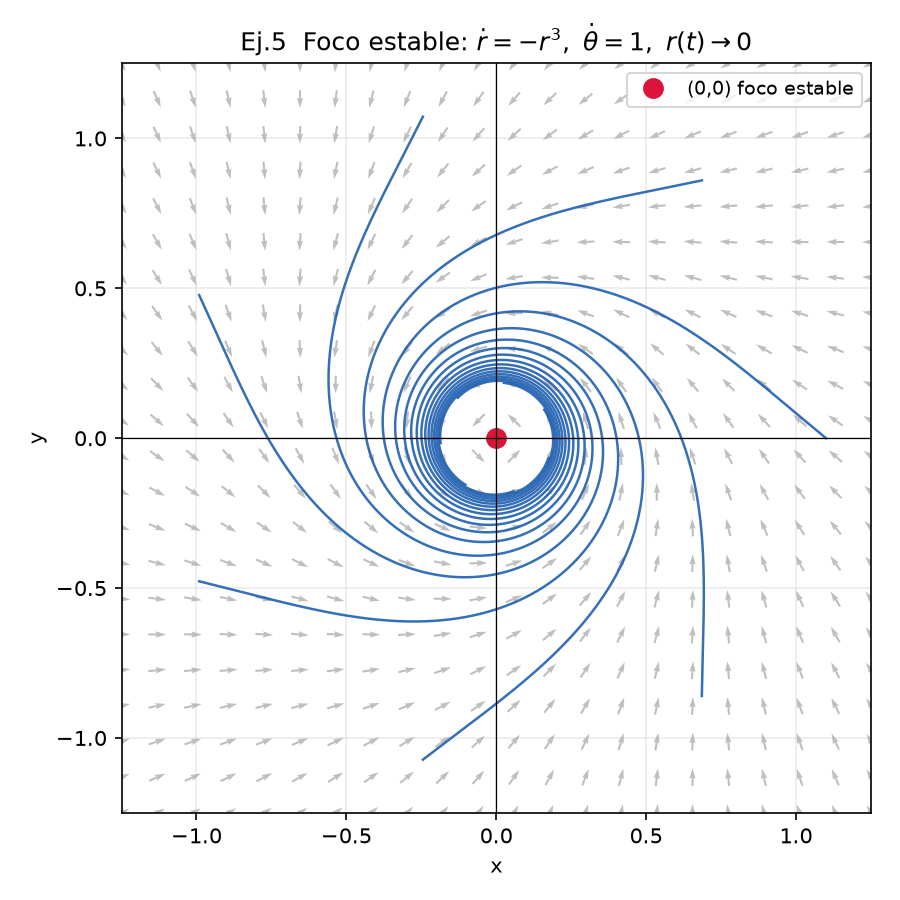
\includegraphics[width=0.60\textwidth]{ej5_espiral.png}\end{figure}

\vspace{2pt}
%==================================================================
\seccion{Resumen}

\begin{center}
\renewcommand{\arraystretch}{1.3}
\begin{tabular}{c l l l}
\toprule
Ej. & Sistema & Equilibrio(s) & Resultado clave\\
\midrule
1 & logístico & $0$ (inest.), $k$ (est.) & $x(t)=\dfrac{k}{1+Ae^{-rt}}$, $t_s\approx16.75$ min\\
2 & lineal & $(0,0)$ & silla; $\lambda=5,-1$; $v=(1,2),(1,-1)$\\
3 & no lineal & $(1,0),(-1,0)$ & no conservativo (div$=2y$); silla y centro\\
4 & Lotka–Volterra & $(0,0),(2,0),(0,3),(1,1)$ & exclusión competitiva (silla en $(1,1)$)\\
5 & no lineal & $(0,0)$ & foco estable; $\dot r=-r^3,\ \dot\theta=1$, $r\to0$\\
\bottomrule
\end{tabular}
\end{center}

\end{document}
